\subsection{Hardware Performance Evaluation}

%This chapter presents the performance evaluation of MCRP on the hardware and testbed. The experiment set ups for TelosB and FlockLab \cite{flocklab} testbed are explained below. Similar to the simulation, MCRP is evaluated using an end-to-end packet delivery performance metric. The results are presented and analysed. 

The real hardware experiments provide the ability to validate MCRP performance in the real wireless channel environments unlike simulation. However, the network's behaviours are complicated to examine as the experiments are not repeatable. The environment condition and the network could be different at each iteration depending on the location, time and channels occupancy. The authors in \cite{homearea} compared the channel occupancy in the office and home environments which potentially can have distinct channel usage. This affects the results differently as the channel conditions could have drastic changes during the run time in the residential environments than in the office environments.

The experiments of MCRP were taken place in both residential and university environments with the same experimental setup.
The results are compared to the single channel case to analyse the MCRP performance in various environments.
A small number of nodes are used in order to confirm that MCRP is working. 
The network consists of 10 nodes; 1 border router and 9 duty cycled nodes. The nodes are placed within at least 1 node's range (approximately 15-80 cm); at the power level of 2 which should have nearly 100\% packet reception given that there is no interference at the range of around 20 cm. 
%The network consists of 7 nodes; 1 border router and 6 duty cycled nodes. The nodes are placed within at least 1 node's range (approximately 15-80 cm); at the power level of 2 which should have nearly 100\% packet reception given that there is no interference at the range of around 20 cm. 
%The reason for this is simplicity to be able to repeat the experiments easily. 
It is done to have a smaller scale of network where all nodes would have the same interference source that affects the nodes. Also, to ensure that the nodes would have at least one hop to the sink to fulfil MCRP criteria in changing channel processes. This experiment can be duplicated to cover a larger scale as the radio has the range that could span over 20-30 metres. 

%\begin{figure}
%\centering
%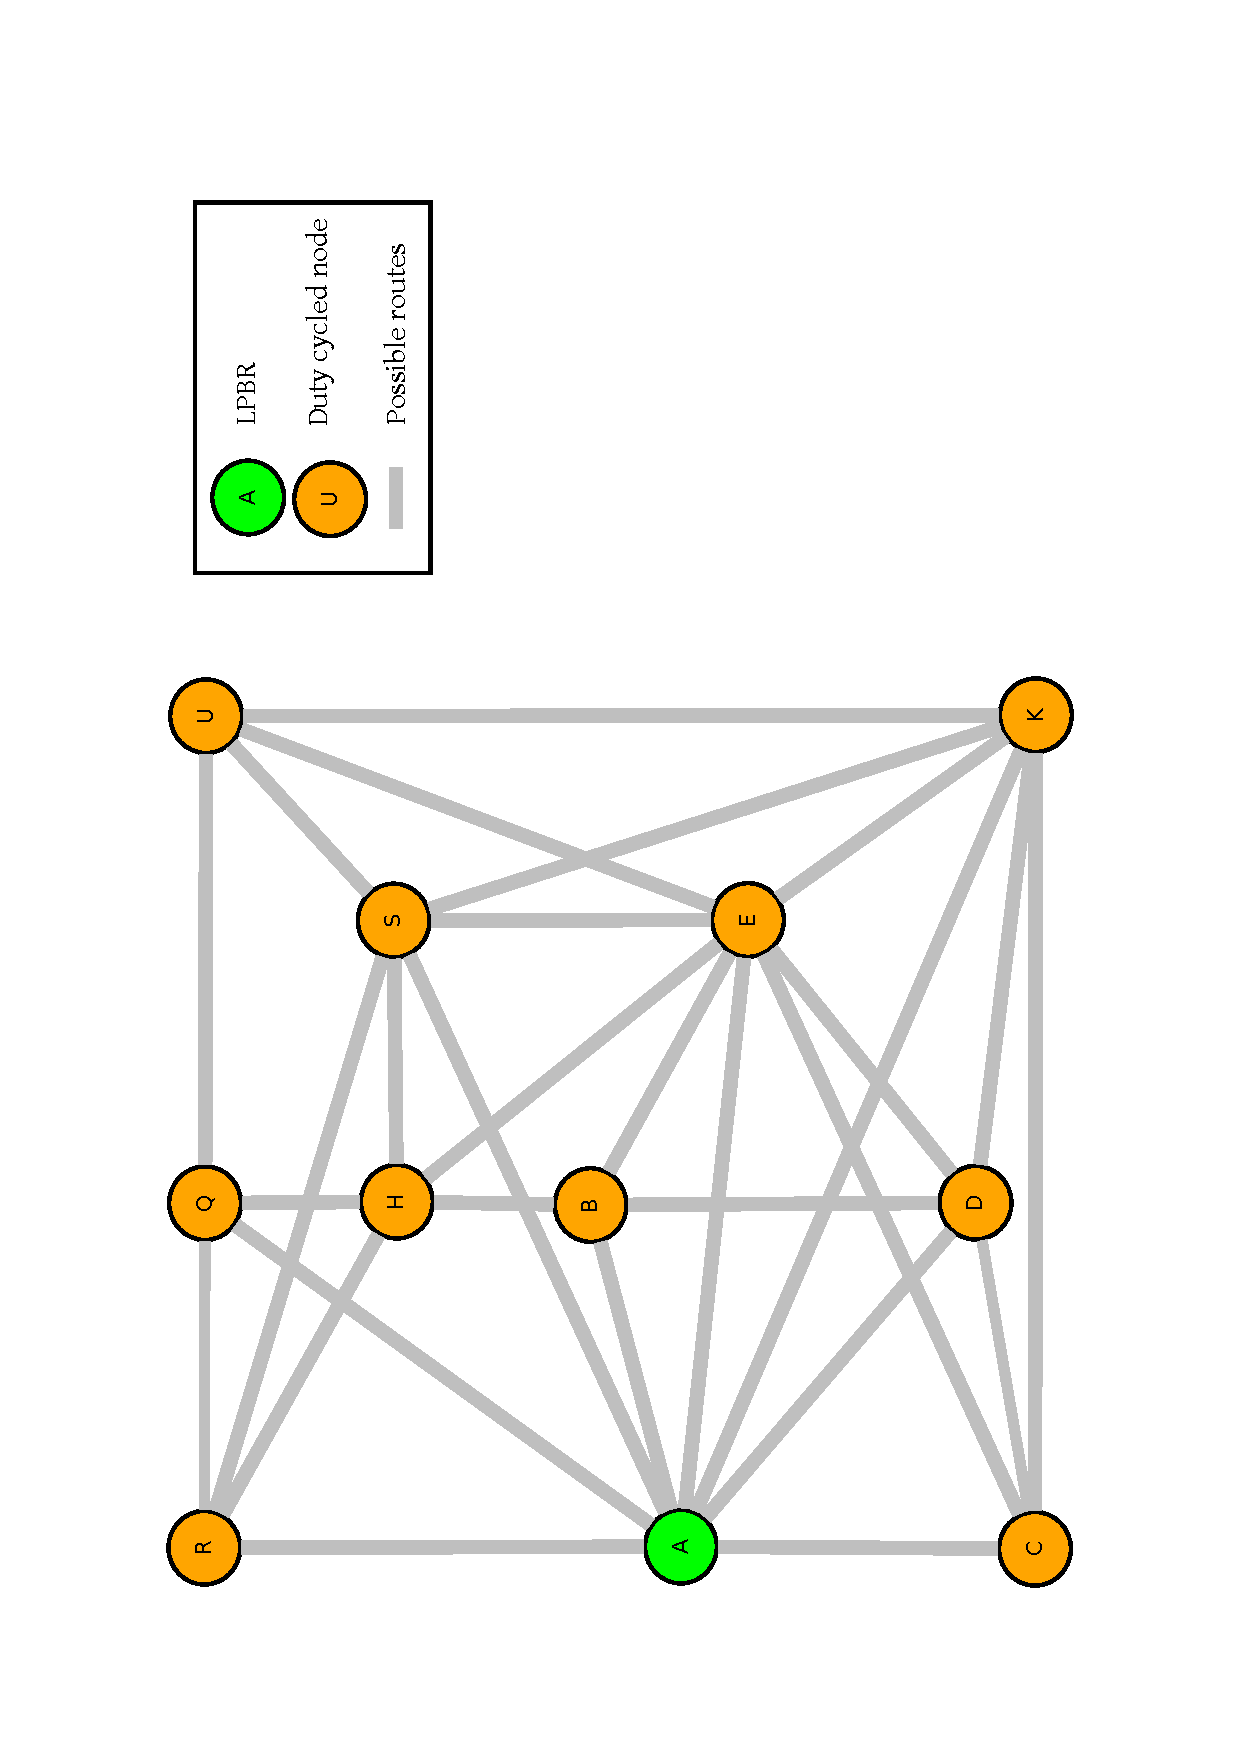
\includegraphics[trim=2cm 2cm 2cm 2cm, clip=true, %totalheight=0.35\textheight, angle=270]{figures/10nodesLayout.pdf}
%\caption{Layout of the real nodes}
%\label{fig_hardwareLayout}
%\end{figure}

The MCRP experiment is run for a duration of 2 hours to send 450 packets, which is 50 packets per node, sending 1 packet per minute for each node. As the nodes are switched on at nearly the same time, RPL is allowed five minutes to set up. MCRP is run for 45 minutes for the channel changes processes. The nodes wait for the MCRP process timer to time out before the nodes can send normal packets. 
%The experiment is then repeated with 11 nodes (1 LPBR, 10 duty cycled nodes) to study the effect that MCRP has with the increased number of nodes. 
The experiments are repeated ten times each. %Figure \ref{fig_hardwareLayout} shows the layout of the nodes and the possible routes that the nodes could choose to get to the LPBR.

%\subsection{Hardware Results}

%%repeatition
%MCRP is compared against the single channel ContikiMAC with RPL.
%Similar to the simulation, the end-to-end packet delivery is used as the performance metric. The proportion of received packets from the sender over multiple hops is plotted with the error bars corresponding to one standard deviation in either deviation to give a measure of repeatability. The values on the x-axis are shifted slightly to avoid overlapping error bars. The experiments of the hardware and testbed are repeated ten times.

Similar to the simulation, the end-to-end packet delivery is used as the performance metric.
The interference could occupy and affect the channels differently at each run. Unlike in the simulation, the RPL tree formation set up is affected by the interference during initialisation. The network could be formed differently at each iteration.

As the nodes are at a close range to the LPBR, some of the nodes could not run the MCRP processes as MCRP requires at least one hop to be able to check the channel condition. However, several nodes were able to run MCRP processes. The tree topology formed differently each time depending on the radio coverage and interference level which affect the RPL ETX value for next hop selection. By increasing the number of nodes and area coverage, it increases the chances that the nodes would have routes to or from which enables MCRP to be executed.

%\begin{figure}
%\centering
%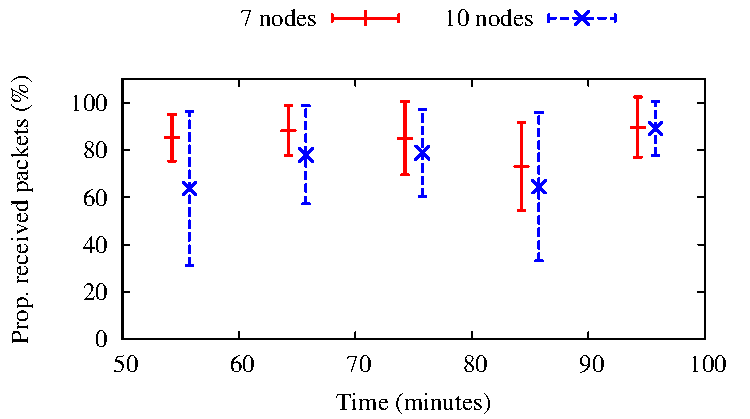
\includegraphics[width=0.45\textwidth]{figures/allNodes.pdf}
%\caption{Real world: Level of packet loss for MCRP}
%\label{fig:hardware}
%\end{figure}

\begin{figure}
\centering
\subfigure[Residential environment]
{\label{fig:hardwareHome}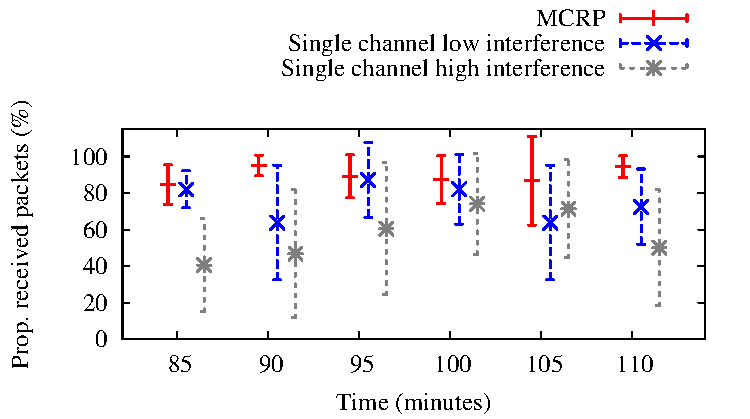
\includegraphics[width=0.45\textwidth]{figures/home.pdf}}
\subfigure[Office environment (UCL)]
{\label{fig:hardwareUCL}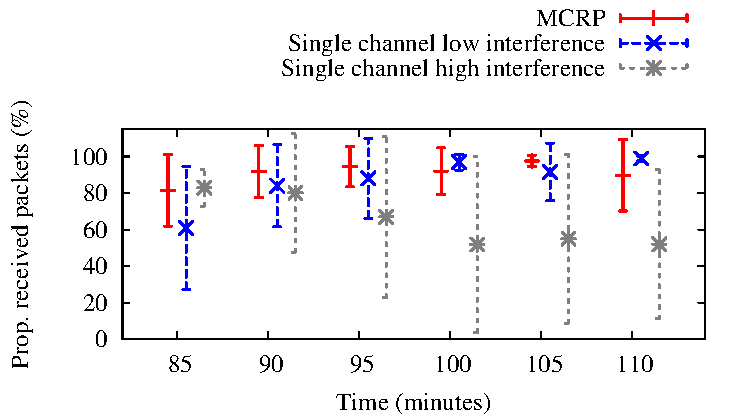
\includegraphics[width=0.45\textwidth]{figures/ucl.pdf}}
\caption{Real world: Level of packet loss for MCRP and single channel}
\label{fig:hardware}
\end{figure}

Figure \ref{fig:hardware} show the results from the experiment in residential and office environments for MCRP compared to a single channel in low and high interference. It can be seen that in both graphs, the number of MCRP received packets vary from approximately 80\% to 90\%. This is because MCRP could hardly find a clear channel for transmissions unlike in the simulation results that show high reception values.
In the single channel case, it can be seen that the results are acceptable in the low interference case. It shows better result in the office environment than in the residential environment as the spectrum usage in the office environment is typically centrally managed. However, both graphs show smaller number of packet reception rate in the extreme interference case compared to the other cases. This shows that MCRP has more advantage than a single channel in extreme interference regardless of the locations. The results are fairly acceptable due to the unpredicted interference occupancy in the 2.4 Ghz frequency band.


%However, in both results, the number of packets loss decreases over time except for at minute 85 before it stabilises again. The reason for this is, the control packets are being sent at the same time (due to trickle timer which enables control packets not to be sent frequently) which resulted in many normal packets to be dropped and lost.

%\begin{figure}
%\centering
%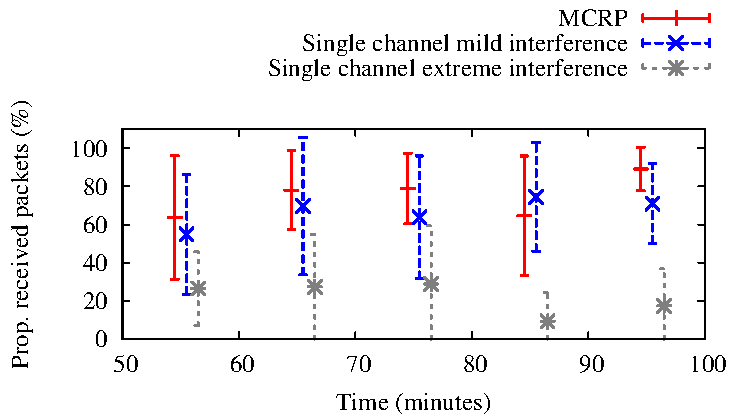
\includegraphics[width=0.45\textwidth]{figures/channels.pdf}
%\caption{Real world: Level of packet loss for MCRP and single channel}
%\label{fig:hardware2}
%\end{figure}

%Figure \ref{fig:hardware2} shows the result of MCRP compared to a single channel in mild to moderate and extreme interference. The single channel with mild interference has the signal strength approximately $-65 dBm$ while the extreme interference is $-40 dBm$. These channels are used for communications to see the effect of the interference channels towards the transmissions. Referring to the interference graph in Figure \ref{fig:interference2}, it can be seen that most channels are occupied except for channel 26 (labelled as 16) which means, MCRP hardly could find a clear channel for transmissions thus the proportion of received packets to be around 50\% to 100\% unlike the simulation results that show high reception values. In the single channel case, it can be seen that the results are acceptable in mild to moderate interference case. However, it shows low packet reception rate in the extreme interference case. This shows that MCRP has more advantage than a single channel in extreme interference. The results are fairly acceptable due to the unpredicted interference occupancy in the 2.4 Ghz frequency band.

%%Comparing to the single channel result, MCRP shows promising result over time. It requires more experiments to be undertaken with some changes to MCRP to run channel changes periodically in order to ensure that it could provide a better number of received packets with small standard deviation than it currently is for higher reliability. 

%///////////

%This chapter presents MCRP in the real world environment. Different than in simulation, the interference level and channels occupancy vary depending on the location. Most of the channels are occupied which makes MCRP appealing than a single channel as it could use several channels for transmissions rather than a single channel that could have high interference over time. The results are fairly acceptable due to the unpredicted interference occupancy in the 2.4 Ghz frequency band. 